%---------------------------------------------------------------------------------------------------
%
%	Edited by: Copyright (c) 2016 Jakub Kúdela
%   Based on: Copyright (c) 2015 Jan Küster
%
%	The MIT License (MIT)
%
%	Permission is hereby granted, free of charge, to any person obtaining a copy
%	of this software and associated documentation files (the "Software"), to deal
%	in the Software without restriction, including without limitation the rights
%	to use, copy, modify, merge, publish, distribute, sublicense, and/or sell
%	copies of the Software, and to permit persons to whom the Software is
%	furnished to do so, subject to the following conditions:
%
%	THE SOFTWARE IS PROVIDED "AS IS", WITHOUT WARRANTY OF ANY KIND, EXPRESS OR
%	IMPLIED, INCLUDING BUT NOT LIMITED TO THE WARRANTIES OF MERCHANTABILITY,
%	FITNESS FOR A PARTICULAR PURPOSE AND NONINFRINGEMENT. IN NO EVENT SHALL THE
%	AUTHORS OR COPYRIGHT HOLDERS BE LIABLE FOR ANY CLAIM, DAMAGES OR OTHER
%	LIABILITY, WHETHER IN AN ACTION OF CONTRACT, TORT OR OTHERWISE, ARISING FROM,
%	OUT OF OR IN CONNECTION WITH THE SOFTWARE OR THE USE OR OTHER DEALINGS IN
%	THE SOFTWARE.
%
%---------------------------------------------------------------------------------------------------


%===================================================================================================
%	DOCUMENT DEFINITION
%===================================================================================================

%we use article class because we want to fully customize the page and dont use a cv template
\documentclass[10pt,a4paper]{article}

%---------------------------------------------------------------------------------------------------
%	ENCODING
%---------------------------------------------------------------------------------------------------

%we use utf8 since we want to build from any machine
\usepackage[utf8]{inputenc}

%---------------------------------------------------------------------------------------------------
%	LOGIC
%---------------------------------------------------------------------------------------------------

% provides \isempty test
\usepackage{xifthen}

%---------------------------------------------------------------------------------------------------
%	FONT
%---------------------------------------------------------------------------------------------------

% some tex-live fonts - choose your own

%\usepackage[defaultsans]{droidsans}
%\usepackage[default]{comfortaa}
%\usepackage{cmbright}
\usepackage[default]{raleway}
%\usepackage{fetamont}
%\usepackage[default]{gillius}
%\usepackage[light,math]{iwona}
%\usepackage[thin]{roboto}
\usepackage{hyperref}

% set font default
\renewcommand*\familydefault{\sfdefault}
\usepackage[T1]{fontenc}

% more font size definitions
\usepackage{moresize}

%---------------------------------------------------------------------------------------------------
%	PAGE LAYOUT  DEFINITIONS
%---------------------------------------------------------------------------------------------------

%debug page outer frames
%\usepackage{showframe}

%define page styles using geometry
\usepackage[a4paper]{geometry}

% for example, change the margins to 2 inches all round
\geometry{top=1.75cm, bottom=-.6cm, left=1.5cm, right=1.5cm}

%use customized header
\usepackage{fancyhdr}
\pagestyle{fancy}

%less space between header and content
\setlength{\headheight}{-5pt}

%customize entries left, center and right
\lhead{}
\chead{\small{
  Axel ROUDAUT $\cdot$
  Ingénieur DevOps en Cybersécurité$\cdot$
  Montpellier, France $\cdot$
  \textcolor{sectcol}{\textbf{\href
  {mailto:axel.roudaut@outlook.com}
  {axel.roudaut@outlook.com}}} $\cdot$
  +33 6 29 76 33 91
}}
\rhead{}

%indentation is zero
\setlength{\parindent}{0mm}

%---------------------------------------------------------------------------------------------------
%	TABLE /ARRAY DEFINITIONS
%---------------------------------------------------------------------------------------------------

%for layouting tables
\usepackage{multicol}
\usepackage{multirow}

%extended aligning of tabular cells
\usepackage{array}
\newcolumntype{x}[1]{>{\raggedleft\hspace{0pt}}p{#1}}

%---------------------------------------------------------------------------------------------------
%	GRAPHICS DEFINITIONS
%---------------------------------------------------------------------------------------------------

%for header image
\usepackage{graphicx}

%for floating figures
\usepackage{wrapfig}
\usepackage{float}
%\floatstyle{boxed}
%\restylefloat{figure}

%for drawing graphics
\usepackage{tikz}
\usetikzlibrary{shapes, backgrounds,mindmap, trees}

%---------------------------------------------------------------------------------------------------
%	Color DEFINITIONS
%---------------------------------------------------------------------------------------------------

\usepackage{color}

%accent color
\definecolor{sectcol}{RGB}{90,90,120}

%dark background color
\definecolor{bgcol}{RGB}{110,110,110}

%light background / accent color
\definecolor{softcol}{RGB}{225,225,225}

%===================================================================================================
%	DEFINITIONS
%===================================================================================================

%---------------------------------------------------------------------------------------------------
% 	HEADER
%---------------------------------------------------------------------------------------------------

% remove top header line
\renewcommand{\headrulewidth}{0pt}

%remove bottom header line
\renewcommand{\footrulewidth}{0pt}

%remove pagenum
\renewcommand{\thepage}{}

%remove section num
\renewcommand{\thesection}{}

%---------------------------------------------------------------------------------------------------
% 	ARROW GRAPHICS in Tikz
%---------------------------------------------------------------------------------------------------

% a six pointed arrow pointing to the left
\newcommand{\tzlarrow}{(0,0) -- (0.2,0) -- (0.3,0.2) -- (0.2,0.4) -- (0,0.4) -- (0.1,0.2) -- cycle;}

% include the left arrow into a tikz picture
% param1: fill color
%
\newcommand{\larrow}[1]{
  \begin{tikzpicture}[scale=0.58]
    \filldraw[fill=#1!100,draw=#1!100!black]  \tzlarrow
  \end{tikzpicture}
}

% a six pointed arrow pointing to the right
\newcommand{\tzrarrow}{ (0,0.2) -- (0.1,0) -- (0.3,0) -- (0.2,0.2) -- (0.3,0.4) -- (0.1,0.4) -- cycle;}

% include the right arrow into a tikz picture
% param1: fill color
%
\newcommand{\rarrow}{
  
\begin{tikzpicture}[scale=0.7]
    \filldraw[fill=sectcol!100,draw=sectcol!100!black] \tzrarrow
  \end{tikzpicture}
}
%---------------------------------------------------------------------------------------------------
%	custom sections
%---------------------------------------------------------------------------------------------------

% create a coloured box with arrow and title as cv section headline
% param 1: section title
%
\newcommand{\cvsection}[1]{
  \vspace{10pt}
  \colorbox{sectcol}{\mystrut \makebox[1\linewidth][l]{
    \larrow{bgcol} \hspace{-8pt} \larrow{bgcol} \hspace{-8pt}
    \larrow{bgcol}\textcolor{white}{\textbf{#1}}\hspace{4pt}
  }}\\
}

%create a coloured arrow with title as cv meta section section
% param 1: meta section title
%
\newcommand{\metasection}[2]{
  \begin{tabular*}{1\textwidth}{p{2.4cm} p{11cm}}
    \larrow{bgcol} \normalsize{\textcolor{sectcol}{#1}}&#2\\[5pt]
  \end{tabular*}
}

%---------------------------------------------------------------------------------------------------
%	 CV EVENT
%---------------------------------------------------------------------------------------------------

% creates a stretched box as cv entry headline followed by two paragraphs
% param 1:	event time i.e. 2014 or 2011-2014 etc.
% param 2:	event name (what did you do?)
% param 3:	institution (where did you work / study)
% param 4:	location
%
\newcommand{\cvevent}[4]{
  \noindent
  \makebox[2.5cm][l]{\textcolor{bgcol}{#1}}%
  \textbf{#2}%
  \hfill
  \textcolor{sectcol}{#3} \textemdash\ \textcolor{sectcol}{#4}

  \vspace{-6pt}
  \textcolor{softcol}{\hrule}
  \vspace{3pt}
}

%
\RequirePackage{relsize}
\RequirePackage{ifthen}
\RequirePackage{listofitems}
\RequirePackage{enumitem}
% Define Custom Colors
\definecolor{cvblue}{rgb}{0.32, 0.68, 0.89}
\definecolor{keywordcolor}{rgb}{0.80, 0.90, 1.0}
% Tech Stack boxes (blue)
\newcommand*{\keyword}[1]{
    \tikz[baseline=(char.base)]{
        \node[rectangle, rounded corners, fill=keywordcolor]
        (char) {\textcolor{black}{#1}};
    }
}

% Core competency color (orange)
\definecolor{corecolor}{rgb}{1.0, 0.75, 0.4}
\newcommand*{\corekeyword}[1]{
    \tikz[baseline=(char.base)]
    {
        \node[rectangle, rounded corners, fill=corecolor]
        (char) {\textcolor{black}{#1}};
    }
}

% creates a stretched box as cv entry detail
% param 1: description
% param 2: core competency (orange)
% param 3: technologies (blue, comma separated)
\newcommand{\cvdetail}[3]{

  % Arrow + Description line
  \begin{tabular*}{\textwidth}{p{0.5cm} p{14.5cm}}
      & \larrow{bgcol} #1\\[-2pt]
  \end{tabular*}

  % Only print core/tech if at least one exists
  \ifthenelse{\equal{#2}{} \AND \equal{#3}{}}%
  {
    % No core and no tech → minimal spacing
    \vspace{7pt}
  }
  {
    % Print core + tech
    \noindent\makebox[0.5cm][l]{}\hspace{10pt}
    \ifthenelse{\equal{#2}{}}{}{\corekeyword{#2}}%
    \ifthenelse{\equal{#3}{}}{}{
        \readlist\keywordlist{#3}
        \foreachitem\word\in\keywordlist{%
            \keyword{\word}%
        }
    }
    \\[-5pt]
  }
}



%---------------------------------------------------------------------------------------------------
% CUSTOM STRUT FOR EMPTY BOXES
%---------------------------------------------------------------------------------------------------
\newcommand{\mystrut}{\rule[-.3\baselineskip]{0pt}{\baselineskip}}

%===================================================================================================
%	DOCUMENT CONTENT
%===================================================================================================
\title{resume}
\begin{document}

% use our custom fancy header definitions
\pagestyle{fancy}
%---------------------------------------------------------------------------------------------------
%	TITLE HEADLINE
%---------------------------------------------------------------------------------------------------
\vspace{-40pt}
% use this for single words, e.g. CV or RESUME etc.
\hspace{-0.25\linewidth}\colorbox{bgcol}{
  \makebox[1.5\linewidth][c]{
    \HUGE{\textcolor{white}{\textsc{Axel Roudaut}}}
    \textcolor{sectcol}{\rule[-1mm]{1mm}{0.9cm}}
    \HUGE{\textcolor{white}{\textsc{Security Data Engineer}}}
  }
}
%---------------------------------------------------------------------------------------------------
% HEADER: META (left) + PHOTO (right)
%---------------------------------------------------------------------------------------------------
\noindent
\begin{tabular*}{\textwidth}{@{\extracolsep{\fill}} p{12cm} r}

% LEFT: META SECTION
\vspace{5pt}
\metasection{Statut :}{DevOps \& Data Engineer en sécurité informatique}
\metasection{Intérêts :}{Data Processing, Automation, Development, System Administration}
\metasection{Formations :}{Ingénieur Télécoms \& Réseaux + Master Cybersecurité - Permis A + B}
\metasection{Activités :}{Escalade, Moto, Skate, Surf, Course à pied, Guitare}


&
% RIGHT: PHOTO
\raisebox{-0.95\height}{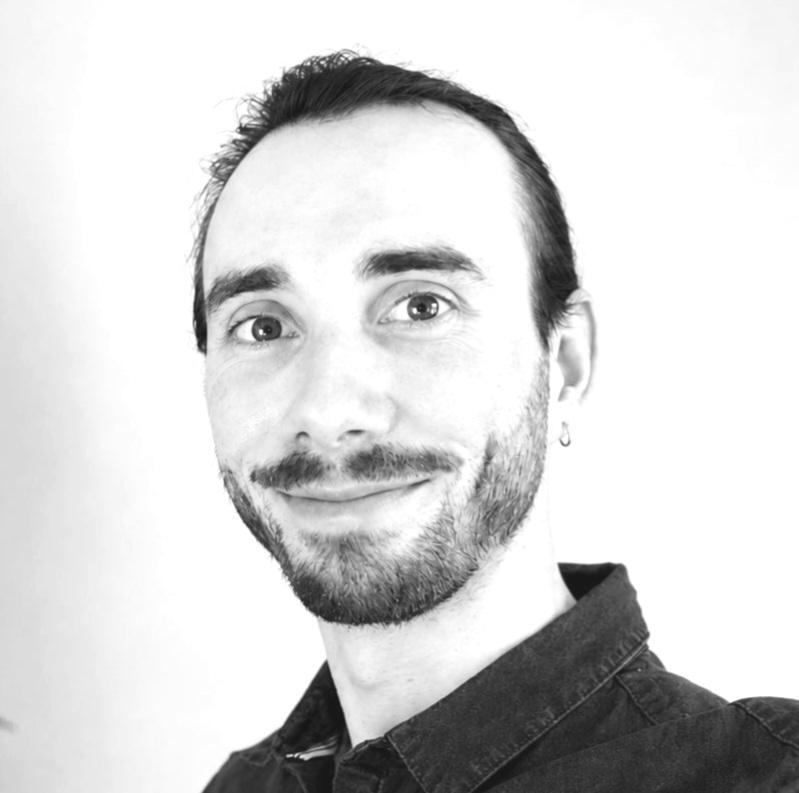
\includegraphics[width=2.9cm]{pic.jpeg}}

\end{tabular*}

%---------------------------------------------------------------------------------------------------
%	SUMMARAY
%---------------------------------------------------------------------------------------------------
\vspace{-12pt}
\cvsection{Résumé}

\textbf{DevOps} et \textbf{Data Engineer} dans le domaine de la Cybersécurité avec \textbf{7+ ans d’expérience} dans la conception et l’exploitation d’infrastructures distribuées et sécurisées (Thales, Ministère des Armées). % codespell:ignore ans
Spécialisé en automatisation CI/CD, orchestration de services et déploiement de plateformes de traitement de données.
Ouvert à des postes DevOps, Data Engineering et Platform Engineering à \textbf{Montpellier} à partir de \textbf{Septembre 2026}.

%===================================================================================================
%	CV SECTIONS AND EVENTS (MAIN CONTENT)
%===================================================================================================

%---------------------------------------------------------------------------------------------------
%	EXPERIENCE
%---------------------------------------------------------------------------------------------------
\cvsection{Expériences}

\cvevent
    {02/22- now}
    {Cybersecurity DevOps Engineer}
    {Thales}
    {Rennes}

\cvdetail
    {Conception et administration de plateformes Kubernetes.}
    {Service Orchestration \& Platform Engineering}
    {Kubernetes, Helm, Docker, Ansible}
\cvdetail
    {Déploiement et maintient d'environnements Linux/Windows de simulation d'attaques.}
    {Infrastructure as Code}
    {VMWare API, Packer, Ansible, Terraform, Powershell}
\cvdetail
    {Optimisation de chaînes de production via des pipelines CI/CD.}
    {DevOps automation}
    {Gitlab CI, Docker, Python, Golang, Bash, Powershell}
\cvdetail
    {Mise en place d'une supervision des infrastructures.}
    {Observability \& Reliability}
    {Prometheus, Grafana, Docker, Ansible}

\cvevent
    {02/19- 02/22}
    {Cyberdefense Data Engineer}
    {Ministère des Armées}
    {Paris}
\cvdetail
    {Conception et configuration d'une architecture de supervision de sécurité (SIEM).}
    {Security Monitoring}
    {Suricata, Auditd, Windows-Security, Sysmon, SIGMA, TheHive}
\cvdetail
    {Implémentation de pipelines de traitement de données en temps réel.}
    {Big Data Processing}
    {Stack Elasticsearch, Kafka, KsqlDB, Apache Spark, HDFS}
\cvdetail
    {Déploiements automatisés et Supervision des infrastructures.}
    {Infrastructure Automation \& Reliability}
    {Docker, Ansible, Gitlab, Prometheus, Grafana}

\cvevent
    {03/18 - 09/18}
    {Stage - Hardware cybersecurity auditing}
    {Trusted Labs}
    {Meudon}
\cvdetail
    {Attaques par canaux cachés électroniques pour des pentests de systèmes embarqués.}
    {Embedded Security}
    {Python, Oscilloscope, Electronic}
\cvdetail
    {Injection de faute sur noyau Android via manipulation d'horloge.}
    {Low-Level System Exploitation}
    {CLKSCREW attack, Bash, Android}

\cvevent
    {06/17 - 08/17}
    {Stage - Cloud Integration Engineer}
    {Altair}
    {Antony}
\cvdetail
    {DevOps Python d'une plate-forme de déploiement d'applications HPC sur clouds publics.}
    {Cloud Platform Engineering}
    {Python, CI/CD, Jenkins, AWS, Azure, GCP, Jira}

%---------------------------------------------------------------------------------------------------
%	EDUCATION SECTION
%---------------------------------------------------------------------------------------------------
\cvsection{Enseignements}

\cvevent
    {2018}
    {Master M2 - Sécurité des Systèmes d'Information et des Réseaux}
    {TLS-SEC}
    {Toulouse}
\cvdetail
    {Cryptography, Assembly, Reverse, Malware, Linux Kernel, Overflow, Network Security}
    {}
    {}

\cvevent
    {2015 - 2018}
    {Diplôme d'Ingénieur - Télécommunications et Réseaux}
    {ENSEEIHT}
    {Toulouse}
\cvdetail
    {Java, C, Assembly, Network Protocols, Cisco, Routing Algorithms, Signal Transmission}
    {}
    {}

\cvevent
    {2017}
    {Échange Erasmus - Big Data and Cyber Security}
    {DCU}
    {Dublin}
\cvdetail
    {Cryptography, Forensic, Network Security, Reverse Engineering, Big Data Hadoop}
    {}
    {}


\cvevent
    {2013 - 2015}
    {Prépa CPGE - Physique et Science de l'Ingénieur}
    {Michelet}
    {Vanves}
%---------------------------------------------------------------------------------------------------
%	ARTIFICIAL FOOTER (fancy footer cannot exceed linewidth)
%---------------------------------------------------------------------------------------------------
\vspace{\fill}
\hspace{-0.25\linewidth}\colorbox{bgcol}{
  \makebox[1.5\linewidth][c]{
    \mystrut \small
    \textcolor{white}{
      \href{https://www.linkedin.com/in/axel-r-72b7131b3}
      {Linkedin}
    } $\cdot$
    \textcolor{white}{
      \href{https://github.com/AxelRoudaut}
      {Github}
    }
  }
}
%===================================================================================================
%	DOCUMENT END
%===================================================================================================
\end{document}
